\documentclass[11pt]{article}
%\documentstyle[amsfonts,11pXSt]{article}
\pdfoutput=1
\usepackage{jheppub}
\usepackage{shuffle}
\usepackage{latexsym}
\usepackage{mathrsfs}
\usepackage{amssymb}
\usepackage{amsmath}
\usepackage{cleveref}
\usepackage{slashed,diagbox,stackrel}
\usepackage[inline]{showlabels}
%\usepackage[hidelinks]{hyperref}
\usepackage[colorinlistoftodos]{todonotes}
\newcommand{\addref}{\todo[color=Red]{Add reference.}}

\usepackage{tikz}
\usepackage{graphicx}
\usepackage{slashed}
%\usepackage[]{showlabels}
%\usepackage{datgtime}
\usepackage{adjustbox}
\usetikzlibrary{shapes.geometric, arrows}
\definecolor{light-gray}{gray}{0.95}
\definecolor{light-grayII}{gray}{0.85}
\usepackage{tikz-feynman} 
%\usepackage
%[%disable.
%color=gray]
%{todonotes} % use with \todo{} or \todo[inline]{} % disable w/ package option [disable]
%\newcommand{\todoin}[1]{\todo[inline]{#1}}
%\newcommand{\todoso}[1]{\todo[color=green]{CITE SOURCE: #1}}

%\newcommand{\addcite}{\todo[color=OrangeRed]{Add citation.}}

%\newcommand{\mathbb}{\Bbb}
\newcommand{\half}{\frac{\scriptstyle 1}{\scriptstyle 2}}
\newcommand{\C}{\mathbb{C}}
\newcommand{\HH}{\mathbb{H}}
\newcommand{\CP}{\mathbb{CP}}
\newcommand{\RP}{\mathbb{RP}}
\newcommand{\PT}{\mathbb{PT}}
\newcommand{\R}{\mathbb{R}}
\renewcommand{\P}{\mathbb{P}}
\newcommand{\bbS}{\mathbb{S}}
\newcommand{\bbD}{\mathbb{D}}
\newcommand{\E}{\mathbb{E}}
\newcommand{\F}{\mathscr{F}}
\newcommand{\cH}{\mathcal{H}}
\newcommand{\scri}{\mathscr{I}}
\newcommand{\M}{\mathbb{M}}
\newcommand{\CM}{\mathscr{M}}
\newcommand{\tCM}{\widetilde{\mathscr{M}}}
\newcommand{\N}{\mathbb{N}}
\newcommand{\T}{\mathbb{T}}
\newcommand{\Z}{\mathbb{Z}}
\newcommand{\p}{\partial}
\newcommand{\dbar}{\bar\partial}
\newcommand{\e}{\mathrm{e}}
\newcommand{\notD}{{\rm D\hskip-0.65em / }}
\newcommand{\D}{\mathrm{D}}
\newcommand{\cC}{\mathcal{C}}
\newcommand{\cX}{\mathcal{X}}
\newcommand{\cD}{\mathcal{D}}
\newcommand{\cE}{\mathcal{E}}
\newcommand{\CF}{\mathcal{F}}
\newcommand{\cG}{\mathcal{G}}
\newcommand{\cK}{\mathcal{K}}
\newcommand{\cI}{\mathcal{I}}
\newcommand{\cA}{\mathcal{A}}
\newcommand{\cL}{\mathcal{L}}
\newcommand{\cM}{\mathcal{M}}
\newcommand{\cT}{\mathcal{T}}
\newcommand{\cO}{\mathcal{O}}
\renewcommand{\P}{\mathbb{P}}
\newcommand{\cY}{\mathcal{Y}}
\newcommand{\cZ}{\mathcal{Z}}
\newcommand{\Pf}{\mathrm{Pf}}
\newcommand{\SL}{\mathrm{SL}}
\newcommand{\End}{\mathrm{End}}
\newcommand{\tr}{\mathrm{tr}}
\newcommand{\sgn}{\mathrm{sgn}}
\newcommand{\SU}{\, \mathrm{SU}}
\newcommand{\GL}{\mathrm{GL}}
\newcommand{\Lie}{{\mathrm{Lie}}}
\newcommand{\diag}{\, \mathrm{diag}}
\newcommand{\rd}{\, \mathrm{d}}
\newcommand{\bs}{\underline{\sigma}}
\newcommand{\bt}{\underline{\tau}}
\newcommand{\bx}{{{\mathbf{x}}}}
\newcommand{\by}{{{\mathbf{y}}}}
\newcommand{\bz}{{\mathbf{z}}}
\newcommand{\bk}{{\mathbf{k}}}
\newcommand{\bV}{{\mathbf{V}}}
\newcommand{\bH}{{\mathbf{H}}}
\newcommand{\DD}{{\rm I\hskip-0.22em D}}
\newcommand{\1}{{\rm 1\hskip-0.25em I}}
\newcommand{\be}{\begin{equation}\label}
\newcommand{\ee}{\end{equation}}
\newcommand{\bea}{\begin{eqnarray}\label}
\newcommand{\eea}{\end{eqnarray}}
\newcommand{\proof}{ \noindent {\bf Proof:} }
\newcommand{\la}{\langle}
\newcommand{\ra}{\rangle}
\newtheorem{defn}{Definition}[section]
\newtheorem{thm}{Theorem}
\newtheorem{proposition}{Proposition}[section]
\newtheorem{propn}{Proposition}[section]
\newtheorem{corollary}{Corollary}[section]
\newtheorem{corol}{Corollary}[section]
\newtheorem{lemma}{Lemma}[section]
\newcommand{\rmk}{\noindent {\bf Remark: }} 
\newtheorem{remark}{Remark}[section]
\newcommand{\example}{\medskip \noindent {\bf Example: } }
%\topmargin0pt
%\headheight0pt
%\headsep0pt
%\oddsidemargin0pt
%\textheight23cm
%\textwidth16cm
\newcommand{\hook}{{\setlength{\unitlength}{10pt}		% adjust hook's size
                  ~ \begin{picture}(.833,.8)
                   \put(-.18,.08){\line(1,0){.7}}
                   \put(.5,.08){\line(0,1){.5}}
                   \end{picture}}}
\begin{document}

\title{Lie Polynomials and a Penrose transform for scattering forms and amplitudes}
\author{Hadleigh Frost and Lionel Mason\\
%}\address{
The Mathematical Institute, University of Oxford,\\
AWB, ROQ, Oxford OX2 6GG, United Kingdom}
%\pacs{99.9x}
%\keywords{perturbative gauge theory, twistor theory}


\abstract{
We review Lie polynomials as a mathematical framework that  underpins  the structure of the so-called double copy relationship between gauge and gravity theories (and a network of other theories besides).  We explain how Lie polynomials naturally arise in the geometry and cohomology of $\cM_{0,n}$ and go on to introduce a Penrose transform between the cotangent bundle $T^*_D\cM_{0,n}$, the bundle of forms with logarithmic singularities on the divisor $D$,  and $\cK_n$ the space of momentum invariants of $n$ massless particles subject to momentum conservation. This gives a natural framework for CHY and ambitwistor-string formulae for scattering amplitudes of gauge and gravity theories.  In particular we show that it gives a natural correspondence between CHY half-integrands and scattering forms, certain $n-3$-forms on $\cK_n$,  introduced by Arkani-Hamed, Bai, He and Yan (ABHY). We  also give a generalization and more invariant description of certain associahedral $(n-3)$-planes in $\cK_n$ introduced by ABHY.  } 

%We develop a Penrose transform based on a correspondence between $T^*_B\cM_{0,n}$,  the bundle of holomorphic 1-forms on the moduli space of $n$ points on $\CP^1$ that have dlog behaviour on the boundary $D$, and the space $\cK_n$ of massless kinematic data (massless Mandelstams).  We use this correspondence to elucidate the geometric structures on $\cK_n$ recently introduced by ABHY.   The most  elementary examples of the transforms take the symplectic volume form on $T^*1_B\cM_{0,n}$ to a family of $(n-3$-forms on $\cK_n$. Other versions coincide with and extend the CHY formulae.  Further examples give rise to the \emph{scattering forms} of \cite{ABHY} and other geometric structures described there.  These  allow a correspondence for CHY `half-integrands' and reformulations of the double copy between gauge and gravity amplitudes.  We present the correspondence in a language that emphasizes the relationships between the geometry of $\cM_{0,n}$, trivalent diagrams and Lie monomials. 



\maketitle

\section{Introduction}
Color-kinematics duality and the double copy \cite{Bern:2008qj, Bern:2010ue} have had a powerful influence on recent developments in scattering amplitudes. They stem from the KLT relations in string theory \cite{Kawai:1985xq} between gravity and Yang-Mills tree-amplitudes and have been devloped as a  tool for the study of multiloop gravity amplitudes and more recently for applications to perturbative classical gravity calculations in connection with gravitational waves \cite{Bern:2019prr}.  Notwithstanding the physical applications, the underlying mathematical results are rather surprising.  There is little hint of such a double copy structure in the classical nonlinear theories involved.
This article develops the underpinning mathematical structures at tree level.  We  build on observations by Kapranov in an after dinner talk \cite{Kapranov} concerning the relevance of Lie polynomials, both in the double copy and in the Parke-Taylor expressions that pervade the subject.   We also build on the recent work by Arkani-Hamed, Bai, He and Yan \cite{Arkani-Hamed:2017mur} that introduces differential forms in the space of kinematic invariants, $\cK_n$.

The first purpose of this work is to provide an elementary exposition of the theory of Lie polynomials as relevant to this topic, and to express standard facts of the double copy in this language.  

We go on to describe the role played by Lie polynomials in the geometry of the moduli space $\cM_{0,n}$ of $n$ points on $\CP^1$, both in describing cycles supported at boundary points of the divisor, and dually in the top degree holomorphic \emph{Parke-Taylor forms}. 


We express these formulae in terms of a geometric correspondence between the 


At tree level, scattering amplitudes are rational functions of momentum invariants, or Mandelstam variables $\cK_n$, and polynomial in invariants that incorporate the polarization data.  The space of momentum invariants is $\cK_n=\R^{n(n-3)/2}$ with coordinates $s_{ij}$, $i,j=1,\ldots , n$, $s_{ij}=s_{ji}$, $s_{ii}=0$ and 
\begin{equation}
\sum_{j=1}^n s_{ij} = 0. \label{conservation}
\end{equation}
These arise from  the definition $s_{ij}=k_i\cdot k_j$ where $k_i$ are $n$ massless momenta in $d$-dimensions subject to momentum conservation $\sum_i k_i=0$.

The key geometric structure in $\cK_n$ as regards amplitudes are the factorization hyperplanes that depend on a subset $I\subset \{1,2,\ldots,n\}$ given by $s_I=0$ where\begin{equation}
s_I:=\sum_{i,j\in I} s_{ij}=\left(\sum_i k_i\right)^2\, .
\end{equation}
We define $|I|$ to be the size of $I$ and $\bar I$ to be its complement so that $s_{\bar I}=-s_I$ by \eqref{conservation}. Locality states that the only singularities of tree amplitudes are simple poles on these hyperplanes.



\section{The double copy and Lie polynomials}

Colour structures for $n$-point  amplitudes are degree $n$ invariant polynomials of weight one in each of the $n$ Lie algebra `colours' of the external particles.  These  naturally arise in Feynman rules as trivalent Feynman diagrams whose vertices are the structure constants of some unspecified Lie algebra.  If we fix the $n$th particle, and an invariant inner product on the Lie algebra, at tree-level, such a polynomial can be realized as the inner product of the $n$th colour with the Lie algebra element with a \emph{Lie polynomial} formed by successive commutators of the $n-1$ other colours working through the diagram back from the $n$th particle. This section reviews material concerning such colour structures in the language of free Lie algebras and Lie polynomials  together with their duality with words formed from permutations of the $n-1$ labels of the first $n-1$ external particles. A classic text on free Lie algebras is \cite{Reutenauer}. We then go on to formulate the BCJ and KLT relations in this framework.

\subsection{An introduction to words, Lie polynomials and trees}

The space of words $W(n-1)$ is the $(n-1)!$-dimensional linear span of  words $a=a_1a_2\ldots a_{n-1}$ where the letters $a_i\in \{1,\ldots,n-1\}$ are all distinct, so that the $a$'a define permutations on $n-1$ letters.  There is a natural inner product on $W(n-1)$ given  on monomials $a$, $b$ by $(a,b)=\delta_{ab}$, i.e., when every letter is the same. 



$Lie(n-1)$ is the vector subspace of $W(n-1)$  generated by all Lie polynomials $\Gamma$ of weight $n-1$ in the $n-1$ variables, $x_1, ... , x_{n-1}$ with weight one in each.  A lie polynomial is formed from iterated commutators of the $x_i$, such as
$$
\Gamma=[x_1,[...,[x_{n-1},x_n]...]] + [x_n,[...,[x_{n-2},x_{n-1}]...]] \in Lie(n-1),
$$
where $[x_i,x_j]=x_ix_j-x_jx_i$ and so on.
 The commutator  is as usual bilinear in its arguments, skew symmetric and satisfies the Jacobi relations
\begin{equation}
[x_i,x_j]=-[x_j,x_i]\, , \qquad [x_i,[x_j,x_k]]+ \mbox {cyclic}=0\, .
\end{equation}
We will see that the dimension of $Lie(n-1)$ is $(n-2)!$.  A possible basis\footnote{Such a basis is also known as a Hall basis \cite{Hall:1950} and is also that introduced by \cite{DelDuca:1999rs}}, the \emph{comb} basis, is given by the Lie monomials of the form
\begin{equation}
\Gamma_{1a}:=[[\ldots [x_{1},x_{a(2)}],...,x_{a(n-2)}],x_{a(n-1)}], \label{comb}
\end{equation}
for all $(n-2)!$ orderings $a$ of $2,\ldots,n-1$. Every Lie monomial in $Lie(n-1)$ can be adjusted up to sign so that $x_1$ appears as the leftmost entry using the skew symmetry of the Lie bracket.


Assuming that the Lie algebra has an invariant inner product, we can take the inner product of $\Gamma$ with an $n$th letter, $x_n$ to give a colour invariant in $n$ letters. 
 We will denote such an invariant degree-$n$ polynomial by $c_\Gamma$.



Such an invariant can be understood as arising from an oriented trivalent connected tree $\Gamma$ with  root $x_n$.  By oriented, we mean each  vertex is oriented, but two oriented diagrams are equivalent if they differ by an even number of orientation reversals at the vertices.  The tree gives a Feynman diagram with structure constants for the Lie algebra at the trivalent vertices oriented by the orientation, which corresponds in turn to the ordering of the Lie brackets appearing in the monomial.  The orientation can also be encoded by expressing the diagram as a planar diagram with  root at $x_n$. Thus for example
%\resizebox{3.5cm}{!}{%
\begin{adjustbox}{width=.8\textwidth
,center}%,float=table}
\begin{tikzpicture}
\begin{feynman}
\vertex (f1);
\vertex [below left=of f1] (b) {\(1\)};
\vertex [above left=of f1] (a) {\(3\)};
\vertex [right = of f1] (i1);
\vertex [right = of i1] (f2);
\vertex [above = of i1] (e) ;
\vertex [above left=of e] (4) {\(4\)};
\vertex [above right=of e] (5) {\(5\)};
\vertex [below right=of f2] (c) {\(6\)};
\vertex [above right=of f2] (d) {\(2\)};
\vertex [left=of f1] {\(
\Gamma= [[[x_1,x_3],[x_4,x_5]],x_2]
=\)};
\diagram* {
(a) --  (f1) --  (b),
(f1) -- (i1) -- (f2),
(i1) -- (e), (e) -- (4),(e) -- (5),
(c) -- (f2) -- (d),
};
\end{feynman}
\end{tikzpicture}
\end{adjustbox}

 In the case of monomial \eqref{comb}, the trivalent diagram $\Gamma_a$ in question is indeed a \emph{comb} (or half-ladder) as its name is intended to express with $x_1$ and $x_n$ at each end, and the remaining $x_i$ being the intermediate teeth in the ordering $a$ as in the following graph %\ref{comb-diagram}
  for the trivial permutation $a=123\ldots n-1$

\begin{center}
\begin{adjustbox}{width=.5\textwidth,center}%,float=table}
  \begin{tikzpicture}[scale=1]
 \draw (0,0) -- (2.25,0) ;
 \draw[dotted, thick] (2.25,0) -- (3.25,0) ;
 \draw (3.25,0) -- (4.5,0);
 \draw (1,0) -- (1,1) ;
 \draw (2,0) -- (2,1) ;
 %\draw (3,0) -- (3,1) ;
 \draw (3.5,0) -- (3.5,1) ;
 \node at (-2,0.7) {$\Gamma_{1a}:=$};
 \node at (-0.4,0) {$1$};
 \node at (4.9,0) {$n$};
 \node at (1,1.4) {$a_2$};
 \node at (2,1.4) {$a_3$};
 %\node at (2.75,0.5,0) {$...$};
 \node at (3.5,1.4) {$a_{n-1}$};
\end{tikzpicture}    
\end{adjustbox}
\end{center}  
  
%\begin{center}
%\includegraphics[width=5cm]{comb.png}\, .
%\label{comb-diagram}
%\end{center}

  The Jacobi identity itself gives the vanishing of the sum of the three four-point graphs corresponding to an $s, t$ and $u$-channel exchange graph.  
  
  \begin{center}
 \begin{tikzpicture}[scale=0.55]
 \draw (0,0) -- (3,0) ;
 \draw (1,0) -- (1,1) ;
 \draw (2,0) -- (2,1) ;
 \node at (-0.4,0) {$1$};
 \node at (3.4,0) {$4$};
 \node at (1,1.4) {$2$};
 \node at (2,1.4) {$3$};
%
 \node at (4.4,0.5) {{\large $+$}};
 \draw (6,0) -- (9,0) ;
 \draw (7,0) -- (7,1) ;
 \draw (8,0) -- (8,1) ;
 \node at (5.6,0) {$1$};
 \node at (9.4,0) {$4$};
 \node at (7,1.4) {$3$};
 \node at (8,1.4) {$2$};
%
 \node at (-2,0.5) {{\large $-$}};
 \draw (-7,0) -- (-4,0) ;
 \draw (-5.5,0) -- (-5.5,0.5) ;
 \draw (-5.5,0.5) -- (-5,1) ;
 \draw (-5.5,0.5) -- (-6,1) ;
 \node at (-7.4,0) {$1$};
 \node at (-3.6,0) {$4$};
 \node at (-6,1.4) {$2$};
 \node at (-5,1.4) {$3$};
  \node at (10.4,0.5) {{\large $\quad=0$}};
\end{tikzpicture}
\end{center}
We will typically denote three Lie polynomials or corresponding graphs that differ only on such a four point subgraph by $\Gamma_s, \Gamma_t$ and $\Gamma_u$ and  we will consequently have
\begin{equation}
\Gamma_s+\Gamma_t+\Gamma_u=0\, .
\end{equation}
It is these relations reduce the dimension of $Lie(n-1)$ to $(n-2)!$ with basis given by the combs $c_{\Gamma_{1a}}$ where $1a$ is an $n-1$- word with first letter 1.   


A tree $\Gamma$ has  \emph{foliage}  given by the  $a$ if it can be realized as a planar tree with external ordering given by the word $an$.  This will be the case if the word $a$  appears in this expansion of $\Gamma$ in $W(n-1)$. We can define
\begin{defn}
The duality between an oriented graph $\Gamma$  and the word $a$ is given by
\begin{equation}
(\Gamma,a)=\begin{cases} \pm1\, , \mbox{ if $\Gamma$ is  planar  with foliage ordered by $(an)$ with $\pm$ induced orientation},\\
 0 \mbox{ otherwise.}\end{cases}
\end{equation}
In terms of words  $(\Gamma,a)=\pm 1$ if $a$ appears with that coefficient in the expansion of its Lie monomial and $0$ otherwise.
\end{defn}
As an application of the notation, note that we can write
\begin{equation}
\Gamma=\sum_a  (\Gamma,a)a \, .\label{gamma-a}
\end{equation}
This follows simply  by expanding out the Lie polynomial based on $\Gamma$ into commutators.


The space of Lie polynomials is $(n-2)!$-dimensional and there are many characterizations of $Lie(n-1)$ as a subspace of $W(n-1)$ \cite{Reutenauer}.  These require the shuffle product

\begin{defn}
The \emph{shuffle product} of a pair of words $b$, $c$ of length $|b|$ and $|c|$  is the  linear combination of words $b\shuffle c$ that is the sum over ordered permutations of the letters of $b$ and $c$ that preserve the original ordering of the letters in $b$ and  $c$. 
\end{defn} 

The following are characterisations of those words   $w\in\subset W(n-1)$ that are in  $Lie(n-1)$:
\begin{propn}\label{Lie-char}
A word $w\in W[n-1]$ is the expansion of a Lie polynomial if either of the following is satisfied:
\begin{enumerate}
\item $(w,a\shuffle b)=0$ for all nontrivial shuffles $a\shuffle b$.
\item The Kleiss-Kuijf relations  \cite{KK1989} 
\begin{equation}
(w, a1b)=(-1)^{|a|}(w,1\bar a\shuffle \ b)\, .
\end{equation}
Here $\bar a$ is the word $a$ in reverse order and $|a|$ the length of $a$.
%together with the $U(1)$ decoupling relation 
%\begin{equation}
%(w,1\shuffle a)=0\, .
%\end{equation}
\end{enumerate}

%\begin{proof}
%We will not prove everything, but refer to the literature:\\
%(1. $\leftrightarrow$ 2.) This is Ree's theorem. It follows by proving that $\delta_\shuffle (AB) =\delta_\shuffle(A)\delta_\shuffle(B)$. \\
%(1. $\leftrightarrow$ 3.) This is a lemma in Schoker. The idea is to study the left bracketing (or comb bracketing) $l(w)$. $P$ is Lie iff $P = l(A)$, for some $A$. The monomial $l(iu)$ contains all words of the form $aib$ where $\bar a \shuffle b$ contains $u$. The sign is $(-1)^{|a|}$, because the length of $a$ is the number of lie bracket flips. So $l(iu) = \sum_{u\in \bar a\shuffle b }(-1)^{|u|} aib$.
%\end{proof}
\end{propn}

See \cite{Reutenauer} chapter 1 for the first (Ree's theorem from 1958) where there are a number of further characterizations.
When $|a|=1$ in the first of these, we obtain the $U(1)$-decoupling relation.

  The last characterization in particular shows that  words $1a$ span $Lie(n-1)^*$ where $a$ is a permutation of $23\ldots n-1$. That the dimension of  $Lie(n-1)$ is $(n-2)!$ with  dual basis given by combs $\Gamma_{1a}$, i.e.\ with $1$ and $n$ at each end follows from
  
  \begin{lemma}
For each $\Gamma$ we can find an $n-2$-word $a_\Gamma$ such that $(\Gamma,1a_{\Gamma})=\pm 1$.  This word is unique for the comb basis \eqref{comb} so that combs and words $1a$ form dual bases of $Lie(n-1)$ and $Lie(n-1)^*$ respectively.
\end{lemma}
\begin{proof}
We can move the letter 1 to the left of each Lie bracket in which it appears using skew-symmetry of the bracket so that it ends up in the first position.  After this process the letter 1 is on the left.  For the comb  basis there is no further freedom as the letter 1 is nested inside all the Lie brackets and so any use of skew symmetry will move 1 away from the first place and there are no further words in the expansion that have the letter 1 on the left. $\Box$
\end{proof}


\subsection{The geometry of $\cK_n$}

The space of Mandelstam variables $\cK_n=\R^{n(n-3)/2}$ with coordinates $s_{ij}$, $i,j=1,\ldots , n$, $s_{ij}=s_{ji}$, $s_{ii}=0$ and 
\begin{equation}
\sum_{j=1}^n s_{ij} = 0. \label{conservation}
\end{equation}
The key geometric structure in $\cK_n$ as regards amplitudes are the factorization hyperplanes that depend on a subset $I\subset \{1,2,\ldots,n\}$ given by $s_I=0$ where\begin{equation}
s_I:=\sum_{i,j\in I} s_{ij}=\left(\sum_i k_i\right)^2\, .
\end{equation}
We define $|I|$ to be the size of $I$ and $\bar I$ to be its complement so that $s_{\bar I}=-s_I$ by \eqref{conservation}. Locality states that the only singularities of tree amplitudes are simple poles on these hyperplanes. 

A key further requirement is that, poles along both $s_I=0$ and $s_J=0$ are only allowed if $I\subset J$ or $\bar J$.
It follows that the allowed pole structure of a contribution to an $n$-point amplitude has poles along at most $n-3$ factorization hyperplanes $s_{I_p}=0$ for $p=1,\ldots ,n-3$.  Such choices are in $1:1$ correspondence with trivalent tree graphs $\Gamma\in \cT$  with $n$-leaves that we will take also, as before in the discussion of Lie polynomials, to be oriented about each vertex. 

\subsection{The double copy from biadjoint scalars to gauge and gravity theories}
The double copy principle is that massless $n$-point tree amplitudes for a large web of important  theories, including many gauge and gravity theories,  can be expressed as a double copy in the form
\begin{equation}
\cM=\sum_\Gamma \frac{N_\Gamma \tilde N_\Gamma}{d_\Gamma}\, .
\end{equation}
Here the denominators
\begin{equation}
d_\Gamma=\prod _{r=1}^{n-3} s_{I_r}
\end{equation}
are the propagator factors associated to the graph $\Gamma$ thought of as a Feynman graph.   Further,  each trivalent diagram $\Gamma$ has a pair of \emph{numerator}  factors   $N_\Gamma$ and $\tilde N_\Gamma$ that are functions of momenta, polarization data, flavour and colour which can therefore include lie polynomials $c_\Gamma$  as invariants.  Such factors are said to be \emph{local} if they are polynomial, i.e., admit no spurious singularities.  

 
The key additional feature required to be a BCJ numerator is that $N_\Gamma$ and $\tilde N_\Gamma$ should represent homomorphisms from  Lie polynomials  to some vector space $V$  of functions of the momenta and polarization and colour data
\begin{equation}
N:Lie(n-1)\rightarrow V
\end{equation}
Thus  for any three graphs $\Gamma_s$, $\Gamma_t$ and $\Gamma_u$ satisfying $[\Gamma_s]+[\Gamma_t]+[\Gamma_u]=0$ as Lie polynomials, we must also have
\begin{equation}
N_{\Gamma_s}+N_{\Gamma_t}+N_{\Gamma_u}=0\, .\label{num-Lie}
\end{equation}

 They are not uniquely determined: given a triple $\Gamma_s$, $\Gamma_t$ and $\Gamma_u$ we can perform the shift 
 $\delta(N_{\Gamma_s}, N_{\Gamma_t}, N_{\Gamma_u})=(s,t,u)A$ for any $A\ni V$.  Such numerators can  be determined from their values on a comb basis $N_{\Gamma_{1a}}$ by
\begin{equation}
N_\Gamma =\sum_{a} (\Gamma ,1a) N_{\Gamma_{1a}}\, .\label{N-basis}
\end{equation}


In the case of Yang mills, since the $c_\Gamma$ are already Lie polynomials, the claim of BCJ \cite{Bern:2008qj} is that
\begin{equation}
\cA=\sum_\Gamma\frac{N_\Gamma^{(\epsilon,k)} c_\Gamma}{d_\Gamma}
\end{equation}
for some \emph{kinematic numerators} $N_\Gamma^{(\epsilon,k)}$ depending on the polarization vectors $\epsilon_i$ and the momenta satisfying \eqref{num-Lie}.  The key nontrivial output of the double copy is that gravity amplitudes are obtained  when $\tilde N_\Gamma=N_\Gamma^{(\epsilon,k)}$. The same numerators determine both 
the colour-ordered Yang-Mills amplitude with order $a$ is then
\begin{equation}
\cA_a = \sum_\Gamma \frac{N_\Gamma (\Gamma,a)}{d_\Gamma }\label{YM-N}
\end{equation}
and gravity amplitudes by
\begin{equation}
\cM = \sum_\Gamma \frac{N_\Gamma N_\Gamma}{d_\Gamma }\, .
\end{equation}



The most basic theory in this framework is the bi-adjoint scalar theory whose colour ordered amplitudes are given by
\begin{equation}
m(a,b):=\sum_\Gamma \frac{(\Gamma,a)(\Gamma,b)}{d_\Gamma}\, .
\end{equation}
and we can introduce two underlying abstract amplitudes for these theories given by
\begin{equation}
m=\sum_\Gamma \frac{\Gamma\otimes \Gamma}{d_\Gamma}\in Lie(n-1)\otimes Lie(n-1) \,, \qquad m_a=\sum_\Gamma\frac{(\Gamma,a)\Gamma}{d_\Gamma}\in Lie(n-1) .
\end{equation}
Substituting \eqref{N-basis} into \eqref{YM-N} we obtain Yang-Mills amplitudes in terms of numerators and $m(a,b)$ by
\begin{equation}
\cA_a=N(m_a)=\sum_b m(a,1b) N_{\Gamma_{1b}}^{(\epsilon,k)}\, ,\label{A-m-N}
\end{equation}
with a similar form for gravity
\begin{equation}
\cM=(N\otimes N)(m) =\sum_{a,b} m(1a,1b)N_{1a}^{(\epsilon,k)}\tilde N_{1b}^{(\epsilon,k)}\,.
\end{equation} 

We briefly remark that the basic kinematic numerators $N^{k,\epsilon}_\Gamma$ for Yang Mills were obtained by \cite{Fu:2017uzt} and other related ones such as $N^{k,k}_\Gamma$ can be created by setting $k_i\cdot \epsilon_j=0$, and $\epsilon_i\cdot \epsilon_j=k_i\cdot k_j$ or $N^{\epsilon,k,m}_\Gamma$ by taking some components of the polarization vectors to be in a higher dimension to the momenta. We thereby obtain, following \cite{Cachazo:2014xea,Casali:2015vta} amplitudes for a variety of theories as
$$
\mbox{ Amplitudes: }\qquad\cM=\sum_\Gamma \frac{N_\Gamma ^l N_\Gamma^r}{d_\Gamma}
$$
as given in table \ref{models}.

\renewcommand{\arraystretch}{1.8}
\begin{table}[h]{%\footnotesize
\centering
\begin{tabular}{|c||l|l|l|l|}
  \hline
  \diagbox{$N^l$}{$N^r$}& $N_\Gamma^{k,\epsilon}$ & $N_{\Gamma}^{k,k}$ & $N_{\Gamma}^{k,\epsilon, m}$ & 
  %$N_{\Gamma}^{k,\epsilon,g}$ &
   $c_{\Gamma} \mbox{ or } (\Gamma,a) $\\ \hline \hline
  $N_\Gamma^{k,\epsilon}$ & E &  & & % &
   \\ \hline 
  $N_{\Gamma}^{k,k}$ & BI & Galileon %&
    &  & \\ \hline  
  $N_{\Gamma}^{k,\epsilon,m}$ & $\stackrel[\text{U}(1)^{m}]{}{EM}$ & DBI & $\stackrel[\text{U}(1)^{m}\times \text{U}(1)^{\tilde m}]{}{EMS}$
  %$\big|_{\text{U}(1)^{m}\times \text{U}(1)^{\tilde m}}
%   &
  & \\
   \hline 
%$N_\Gamma^{k,\epsilon,g}$ & EYM & ext.\ DBI & $\stackrel[\text{SU}(N)\times \text{U}(1)^{\tilde m}]{}{EYMS}$ & $\stackrel[\text{SU}(N)\times \text{SU}(\tilde N)]{}{EYMS}$ & \\ \hline  
  $c_\Gamma \mbox{ or } (\Gamma,a)$ & YM &  Nonlinear $\sigma$ & $\stackrel[\text{SU}(N)\times \text{U}(1)^{\tilde m}]{}{EYMS}$ & 
 % $\stackrel[\text{SU}(N)\times \text{SU}(\tilde N)]{}{gen.\ YMS}$ &
  $\stackrel[\text{SU}(N)\times \text{SU}(\tilde N)]{}{Biadjoint\; Scalar}$\\ \hline 
 \end{tabular}}
 \caption{Theories arising from the different choices of numerators.} \label{models}
\end{table}

We cannot simply invert \eqref{A-m-N} to obtain the $N_{1b}$ as $m(1a,1b)$ is not invertible. Indeed, 
all theories that can be expressed in this double-copy format with one explicit Lie polynomial factor satisfy the fundamental BCJ relations \cite{Bern:2008qj}.  There are many forms of the relations,  one version being, for a word\footnote{This is eq 3.8 of \cite{Cachazo:2012} together with the use of the $U(1)$-decoupling identity in the bracketed term.} $a\in W(n-2)$
\begin{equation}
\sum_{bc=a} s_{i,b_{|b|}} m((i\shuffle b)c)  =0\, ,
%.\end{equation} \begin{equation} \sum_{bc=a}s_{b\,n-1} m(b (n-1) c)=0\, ,
 \qquad 
\mbox{ where } \quad s_{b, k}:=\sum_{i=1}^{|b|} s_{b_i\, k}\, .
\end{equation}

Thus  \eqref{A-m-N} determines the $N_{1a}$ only up to the addition of multiples of the BCJ relations.  This freedom can be used to set all but $(n-3)!$ of the $N_{1a}$ to zero, but this is at the expense of requiring numerators that are rational rather than polynomial in the momenta which will then have spurious poles.  



\section{Trees and words in $\cM_{0,n}$}
In this section we consider the homology and cohomology of $\cM_{0,n}^\#$ the space of $n$ distinct points on the Riemann sphere $\CP^1$ up to Mobius transformations, together with its Deligne Mumford compactification $\cM_{0,n}$. \begin{center}
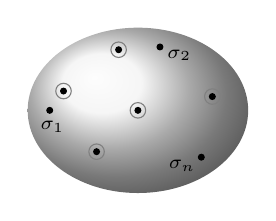
\begin{tikzpicture} [scale=3.5]%Riemann Sphere
\shade[shading=ball, ball color=light-gray] (3.6,1.5) circle [x radius=0.4, y radius=0.3];
%  \draw (3.6,1.5) circle [x radius=0.4, y radius=0.3];
  \draw [fill] (3.33,1.57) circle [radius=.3pt];
  \draw [gray] (3.33,1.57) circle [radius=.8pt];
  \draw [fill] (3.28,1.5) circle [radius=.3pt];
  \node at (3.29,1.44) {\scriptsize $\sigma_1$};
  \draw [fill] (3.45,1.35) circle [radius=.3pt];
  \draw [gray] (3.45,1.35) circle [radius=.8pt];
  %\draw [fill] (3.8,1.43) circle [radius=.3pt];
  \draw [fill] (3.87,1.55) circle [radius=.3pt];
  \draw [gray] (3.87,1.55) circle [radius=.8pt];
  \draw [fill] (3.6,1.5) circle [radius=.3pt];
  \draw [gray] (3.6,1.5) circle [radius=.8pt];
  \draw [fill] (3.53,1.72) circle [radius=.3pt];
  \draw [gray] (3.53,1.72) circle [radius=.8pt];
  \draw [fill] (3.68,1.73) circle [radius=.3pt];
  \node at (3.75,1.7) {\scriptsize $\sigma_2$};
  \draw [fill] (3.83,1.33) circle [radius=.3pt];
  \node at (3.76,1.3) {\scriptsize $\sigma_n$}; 
 \end{tikzpicture}
\end{center}


We will see that Lie polynomials and their duals arise in the homology and cohomology of $\cM_{0,n}$.   We have
\begin{equation}
H_{n-3}(\cM_{0,n}-D)=Lie(n-1), 
\end{equation}
and construct cycles corresponding to each $\Gamma$.  Dually we have
\begin{equation}
\Gamma(\cM_{0,n},\Omega^{n-3}_D)=Lie(n-1)^*.
\end{equation}
This dual space is generated by the familiar Parke-Taylor forms. 

\subsection{The cohomology of $\cM_{0,n}$ and Parke-Taylors} 

The dimensions of the cohomology groups of $\cM_{0,n}^\#$
are given by  the Poincar\'e polynomial\footnote{Arnol'd \cite{Arnold}
computes the Poincar\'e polynomial of the cohomology of the configuration space $M_{n-1}$ of $n-1$ points in $\C$.  This can be obtained inductively via  the fibration $M_{k}\rightarrow M_{k-1}$ with fibre $\C-\{\sigma_1,\ldots,\sigma_{k-1}\}$ giving factors of $(1+(k-1)t)$. For $\cM_{0,n}$ one needs to take the quotient by $\C^*\ltimes \C$ to get $\cM_{0,n}$.   Arnol'd's formula for the Poincar\'e polynomial of $M_{n-1}$  must therefore be divided  by $1+t$ to obtain the formula here.}  
\begin{equation}
P(t) :=\sum_i \dim (H^i(\cM^\#_{0,n}))\,t^i=\prod_{k=2}^{n-2} (1+kt)\, .
\end{equation}
The cohomology ring is generated by the $\rd \log \sigma_{ij}$ in the standard gauge fixing subject to the quadratic relations 
\begin{equation}
\frac{d\sigma_{ij}}{\sigma_{ij}} \wedge \frac{d \sigma_{jk}}{\sigma_{jk}} +
\frac{d\sigma_{jk}}{\sigma_{jk}} \wedge \frac{d\sigma_{ki}}{\sigma_{ki}} +
\frac{d\sigma_{ki}}{\sigma_{ki}} \wedge \frac{d\sigma_{ij}}{\sigma_{ij}} =0\, . \label{schouten}
\end{equation}
This gives the dimension of $\Gamma(\Omega_D^1)$ as $\sum_{k=2}^{n-2}=n(n-3)/2$ as claimed earlier. Our focus will be on  top degree holomorphic forms and their dual cycles.  

 The above shows that the cohomology $H^{n-3}(\cM_{0,n}^\#)=\Gamma (\cM_{0,n},\Omega^{n-3}_D)$ and has dimension $(n-2)!$.  A natural spanning set for 
 $\Gamma(\Omega^{n-3}_D)$ is provided by the Parke-Taylor forms  
\begin{equation}
PT(123\ldots n)=\frac{1}{\mathrm{Vol}SL(2)} \prod_{i=1}^n \frac{d\log \sigma_{i\, i+1}}{2\pi i}\, .
\end{equation}
In our gauge fixing 
\begin{equation}
\frac{1}{\mathrm{Vol}SL(2)}=\frac{(2\pi i)^3\sigma_{1\, n-1}\sigma_{n-1\, n}\sigma_{n1}}{d\sigma_1d\sigma_{n-1} d\sigma_n}
\end{equation}
yielding now for a general choice of permutation $a$ of $1,\ldots ,n-1$
\begin{equation}
PT_a:=PT(a n)=\frac{d^{n-3}\sigma }{\prod_{i=1}^{n-2} 
%\frac{1}{
\sigma_{{a(i)\, a(i+1)}}} \, , \qquad d^{n-3}\sigma:=\frac{1}{(2\pi i)^{n-3}}\prod_{i=2}^{n-2} d\sigma_i\, .
\end{equation}
The Parke-Taylor forms can be acted on by permutations, but it is clear that cyclic permutations act trivially so we can always take $n$ to be the last entry. Following Proposition \ref{Lie-char}, $PT_a$ satisfy the shuffle relations identically $PT_{b\shuffle c}=0$ for $b,c$ nontrivial.  Furthermore the Kleiss-Kuijf relations allows one to take $1$ as the first entry yielding a basis for the $(n-2)!$-dimensional space $\Gamma(\M_{0,n},\Omega^{n-3}_D)$. It is naturally expressed in terms of permutations  by permuting the remaining entries. Following \cite{Reutenauer}, we will denote these as words $a$ in the letters $\{1,2,\ldots ,n-1\}$. The Kleiss Kuijf basis is made up of $PT_a$ where the \emph{word} $a$ is a permutation of $\{1,\ldots, n-1\}$ that fixes 1.



\subsection{Homology of $\cM_{0,n}$}
We will adopt the traditional normalization of  the $\sigma_i$ under Mobius transformations so that $(\sigma_1,\sigma_{n-1},\sigma_n)=(0,1,\infty)$. This has a large open cell $\cM_{0,n}^\#$ on which the $n$ points are distinct, together with the boundary divisor $D$ stratified by the codimension-1 loci $D_I$ for subsets $I\subset\{1,\ldots,n\}$, where the $\sigma_i$ for $i\in I$  bubble off onto a new $\CP^1$ attached to the first by a node:

\begin{center}

$I$\qquad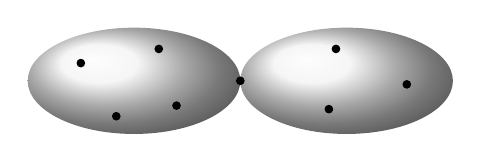
\begin{tikzpicture}[scale=4.5]
 %factorised 
 \shade[shading=ball, ball color=light-gray] (4.75,1.7) circle [x radius=0.3, y radius=0.15];
 \shade[shading=ball, ball color=light-gray] (5.35,1.7) circle [x radius=0.3, y radius=0.15];
 % \draw [dashed,red] (4.82,1.79) to [out=60, in=180] (5.07,1.95) to [out=0, in=120] (5.32,1.79);
  \draw [fill] (4.6,1.75) circle [radius=.3pt];
 \draw [fill] (4.7,1.6) circle [radius=.3pt];
  \draw [fill] (4.87,1.63) circle [radius=.3pt];
  \draw [fill] (5.3,1.62) circle [radius=.3pt];
  \draw [fill] (5.52,1.69) circle [radius=.3pt];
  \draw [fill] (4.82,1.79) circle [radius=.3pt];
  \draw [fill] (5.32,1.79) circle [radius=.3pt];
  \draw [fill] (5.05,1.7) circle [radius=.3pt];
\end{tikzpicture} \qquad $\bar I$\end{center}

On intersections of strata we will have bubbles into more components connected at nodes. In order to see a stratum $D_I$ directly, we need to introduce dihedral coordinates. These require the choice of an ordering for which $I$ is a consecutive subset.  In the case of the standard ordering we define the \emph{chord coordinates}
\begin{equation}
u_{ij}=\frac{\sigma_{i\,j-1}\sigma_{i-1\, j}}{\sigma_{ij}\sigma_{i-1\, j-1}}\, , \qquad j>i+1\, ,\qquad \sigma_{ij}=\sigma_i-\sigma_j\, .
\end{equation}
When $I=\{1,2,\ldots ,|I|\}$, with $|I|$ being the size of $I$, we take  $u_{1\, i}$, $i=3,\ldots,n-1$ as our coordinates on  $\cM_{0,n}$ and in these coordinates, the $D_I$ are given by $u_{1\,|I|+1}=0$.  To see this we need the `non-crossing identity'
\begin{equation}
u_{ij}=1-\prod_{(k,l)\in (i,j)^c} u_{kl}\, , \label{non-cross}
\end{equation}
where for $k<l$, $(k,l)\in (i,j)^c$ means that the diagonal $(k,l)$ of the polygon with vertices $\{1,\ldots,n\}$ crosses the diagonal $(i,j)$.  This implies that on $u_{1\, |I|+1}=0$, $u_{ij}=1$ for $i\in I-1$ and $j\in \bar I-\{|I|+1\}$ as then $u_{1\,|I|}\in (i,j)^c$ and this forces $\sigma_{i}\rightarrow 0$ for $1<i\in I$ in our gauge fixing with the interpretation that the $\sigma_i$ for $i\in I$ have bubbled off into their own Riemann sphere (fixing instead $(\sigma_1,\sigma_2,\sigma_n)=(0,1,\infty)$ would instead have left $\sigma_i, i\in I$ finite but sent $\sigma_i, i\in \bar I$ to $\infty$.
An often remarked  feature of the boundary divisor is its recursive structure
\begin{equation}
 D_I=\cM_{0,|I|+1}\times \cM_{0,|\bar I|+1}\, ,
\end{equation}
as the two components of the nodal sphere have $|I|+1$ and $|\bar I|+1$ marked points respectively with the additional points being the node that connects them.   



It is clear that two divisor components $D_I, D_J$ can only intersect if $I\subset J$ or $I\subset J^c$ the complement of $J$ as otherwise the $I$ cannot separate a bubbled-off component of $J$.  Iterating we see that the maximal intersection of boundary components are points $D_\Gamma$ that arise as the $n-3$-fold intersection of $n-3$ components $D_{I_p}$ that are mutually compatible. Such compatible intersections are therefore naturally in $1:1$ correspondence with trivalent diagrams $\Gamma$ as before in the $n-3$-fold intersection of compatible factorization hyperplanes in $\cK_n$.

These dimension-0 strata $D_\Gamma$ naturally give rise to cycles $T_\Gamma$ 
$H_{n-3}(\cM_{0,n}^\#)$ given by $n-3$-dimensional tori. To be more explicit, $\Gamma$  has $n-3$ internal propagators with the $p$th determining the partition of $\{1,\ldots, n\}=I_p\cup \bar I_p$  of leaves on either side of the propagator (which corresponds to a node on the curve separating it into the two corresponding components).  To present $T_\Gamma$ explicitly, choose a dihedral ordering so that $\Gamma$ is planar.  Relative to this we can introduce the chord coordinates $u_{ij}$. (A given tree, $\Gamma$, is compatible with $2^{n-3}$ distinct dihedral structures. Any choice of dihedral structure defines the same class in homology.) The propagators determine  $n-3$ of these chords,  $u_{I_p}$, $p=1,\ldots , n-3$ whose vanishing gives $D_\Gamma$.
Then the cycle  is defined by 
\begin{equation}
T_\Gamma=\{|u_{I_1}|=|u_{I_2}|=\ldots=|u_{I_{n-3}}|=\epsilon\}\subset \cM_{0,n}\, , \label{cycle}
\end{equation}
for some small $\epsilon$.  
We need to furthermore define an orientation for $T_\Gamma$.  Each circle defined in \eqref{cycle} is oriented anticlockwise in its complex plane $u_{I_p}$ around the origin.  The full orientation will then be determined implicitly by.

These cycles are not linearly independent in homology.  This is most easily seen at four points where $\cM^\#_{0,n}=\CP^1-\{0,1,\infty\}$,
with boundary points  $D_{s}=0$, $D_{t}=1$, and $D_{u}=\infty$; the notation is intended to suggest four point graphs with propagators in the $s$, $t$ and $u$ channels (i.e., with $s=s_{12}, t=s_{14}$, and $u=s_{13}$). It is then easily seen that the three contours around these points add up to zero in homology
\begin{equation}
[T_{s}]+[T_{t}]+[T_u]=0\, .
\end{equation}
This gives the  expected two-dimensions for $H_1(\cM^\#_{0,4})$. 


\begin{center}
 \begin{tikzpicture}[scale=0.4]
 \draw (0,0) -- (3,0) ;
 \draw (1,0) -- (1,1) ;
 \draw (2,0) -- (2,1) ;
 \node at (-0.4,0) {$\scriptstyle{1}$};
 \node at (3.4,0) {$\scriptstyle{4}$};
 \node at (1,1.5) {$\scriptstyle{2}$};
 \node at (2,1.5) {$\scriptstyle{3}$};
%
 \node at (4.4,0.5) {{ $+$}};
 \draw (6,0) -- (9,0) ;
 \draw (7,0) -- (7,1) ;
 \draw (8,0) -- (8,1) ;
 \node at (5.6,0) {$\scriptstyle{1}$};
 \node at (9.4,0) {$\scriptstyle{4}$};
 \node at (7,1.5) {$\scriptstyle{3}$};
 \node at (8,1.5) {$\scriptstyle{2}$};
%
 \node at (-2,0.5) {{ $-$}};
 \draw (-7,0) -- (-4,0) ;
 \draw (-5.5,0) -- (-5.5,0.5) ;
 \draw (-5.5,0.5) -- (-5,1) ;
 \draw (-5.5,0.5) -- (-6,1) ;
 \node at (-7.4,0) {$\scriptstyle{1}$};
 \node at (-3.6,0) {$\scriptstyle{4}$};
 \node at (-6,1.5) {$\scriptstyle{2}$};
 \node at (-5,1.5) {$\scriptstyle{3}$};
  \node at (10.4,0.5) { $\quad=0$};
  \end{tikzpicture} $\; \leftrightarrow\;$
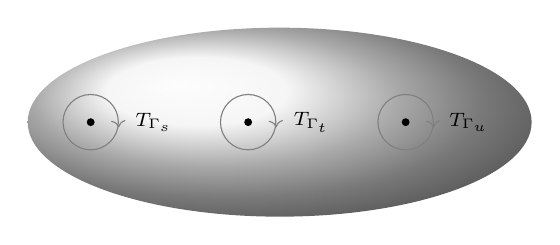
\begin{tikzpicture} [scale=4]%Riemann Sphere
\shade[shading=ball, ball color=light-gray] (3.6,0) circle [x radius=0.8, y radius=0.3];
%  \draw (3.6,0) circle [x radius=0.8, y radius=0.3];
%  \draw [fill] (3.33,1.57) circle [radius=.3pt];
\draw [gray, decoration={markings, mark=at position 0.01 with {\arrow{<}}}, postaction={decorate}] (3,0) circle [radius=2.5pt];
%  \draw [gray] (3,0) circle [radius=2pt];
  \draw [fill] (3,0) circle [radius=.3pt];
  \node at (3.2,0) {\scriptsize $T_{\Gamma_s}$};
 % \draw [fill] (3.45,1.35) circle [radius=.3pt];
 % \draw [gray] (3.45,1.35) circle [radius=.8pt];
  %\draw [fill] (3.8,1.43) circle [radius=.3pt];
%  \draw [fill] (3.87,1.55) circle [radius=.3pt];
%  \draw [gray] (3.87,1.55) circle [radius=.8pt];
%  \draw [fill] (3.6,1.5) circle [radius=.3pt];
%  \draw [fill] (3.53,1.72) circle [radius=.3pt];
%  \draw [gray] (3.5,0) circle [radius=2pt];
\draw [gray, decoration={markings, mark=at position 0.01 with {\arrow{<}}}, postaction={decorate}] (3.5,0) circle [radius=2.5pt];
  \draw [fill] (3.5,0) circle [radius=.3pt];
  \node at (3.7,0) {\scriptsize $T_{\Gamma_t}$};
\draw [gray, decoration={markings, mark=at position 0.01 with {\arrow{<}}}, postaction={decorate}] (4,0) circle [radius=2.5pt];
%  \draw [gray] (4,0) circle [radius=2pt];
  \draw [fill] (4,0) circle [radius=.3pt];
  \node at (4.2,0) {\scriptsize $T_{\Gamma_u}$}; 
 \end{tikzpicture}.
\end{center}

 This relation will arise similarly on any $\CP^1$  component of $D$:  when four given trees are attached to the four legs of either an $s,t$ or $u$ exchange diagrams, we form trees $\Gamma_s, \Gamma_t$ and $\Gamma_u$  that sit inside such a $\CP^1 \subset D$.  The same argument on this $\CP^1$ shows that 
\begin{equation}
[T_{\Gamma_s}]+[T_{\Gamma_t}]+[T_{\Gamma_u}]=0\, .\label{stu-id}
\end{equation}

Thus
\begin{lemma}
There is a canonical identification 
\begin{equation}
 H_{n-3}(\cM_{0,n})= Lie(n-1)
\end{equation}
given by identifying the cycle $T_\Gamma$ with the monomial $P_\Gamma$ corresponding to the planar tree $\Gamma$ rooted at $n$.
\end{lemma}

\begin{proof}
The main task is to see that the skew symmetry is correctly encoded by the orientation and that the Jacobi identity by the $stu$-identity \eqref{stu-id} but these are clear. $\Box$
\end{proof}


\smallskip




Dually we have 
\begin{propn}\label{T-PT-pairing}
The natural integration pairing  between $H_{n-3}(\cM^\#_{0,n})$ and $\Gamma(\cM_{0,n},\Omega^{n-3}_D)$ is \begin{equation}
(T_\Gamma,PT_a):=\int_{T_\Gamma}PT_a =(\Gamma,a)
\end{equation}
i.e., $\pm 1$ if $\Gamma $ is planar for the ordering $a$, otherwise zero. \end{propn}

\begin{proof}
The standard Parke-Taylor form can be written as 
\begin{equation}
PT(12\ldots n)=\prod_{i=3}^{n-1} \frac{1}{2\pi i}d\log \frac{ u_{1i}}{1- u_{1i}}\, .\label{comb-PT}
\end{equation}
If $T_\Gamma=\{|u_{1i}|=\epsilon, i=3,\ldots ,n-1\}$, i.e.\ $\Gamma $ is the standard comb, the pairing then obviously gives  1. If  we interchange $2$ and $3$ in $\Gamma$ the $u_{13}$ part of the contour will be $|\frac1{u_{13}}|=\epsilon$ but the Parke-Taylor has no pole at $u_{13}=\infty$ so the pairing will give zero. The $stu$ identity will then give $- 1$ for the planar graph for which $2,3$ connect to a vertex, whose third propagator  attaches to the standard comb with one fewer teeth (this is contour $|u_{13}-1|=\epsilon$) that encircles the manifest pole with residue $-1$ at $u_{13}=1$.  The general planar graph compatible with the ordering can be obtained by such $stu$ moves acting on the propagator between $i-1$ and $i$ by studying such moves on each $u_{1i}$-plane. $\Box$
\end{proof}




\section{A Penrose transform for amplitudes}

Our  starting point is the observation that $\cK_n$ also arises naturally from the geometry of $\cM_{0,n}$ the Deligne-Mumford compactification of the moduli space of $n$ points $\sigma_i$, $i=1,\ldots,n$ on $\CP^1$ up to M\"obius transformations.  

Our `twistor space' for the Penrose transform will be $\T=T^*_D \cM_{0,n}$, the total space of the bundle of holomorphic 1-forms on $\cM_{0,n}$ with $d\log $ singularities on $D$. The relationship with $\cK_n$ is given by 
\begin{equation}
\cK_n=\Gamma({\cM_{0,n}},T^*_D )\, .
\end{equation}
This correspondence can be expressed by considering $d \log $ of the
 Koba-Nielsen factor \begin{equation}
 KN:=\prod_{i<j} \sigma_{ij}^{s_{ij}}\, , \qquad \sigma_{ij}=\sigma_i-\sigma_j\, .
 \end{equation}
  This gives the general section of $\tau\in \Gamma(T^*_D \cM_{0,n}) $ as 
 \begin{equation}
\tau=\sum_iE_id\sigma_i:= \sum_{i<j} s_{ij}d \log \sigma_{ij}\, , \qquad E_i=\sum_j\frac{s_{ij}}{\sigma_{ij}}\, .
 \end{equation}
Our normalizations $(\sigma_1,\sigma_{n-1},\sigma_n)=(0,1,\infty)$ gives the triviality of $d\log \sigma_{in}$ and $d\log \sigma_{1\,n-1}$ giving the correct dimensionality of the $d\log\sigma_{ij}$ basis. We remark that the vanishing of the $E_i$ are the \emph{scattering equations}.

To more clearly demonstrate the $d\log$ behaviour on $D$, given the choice of the standard ordering, we can also represent the Koba Nielsen factor as 
\begin{equation}
KN=\prod_{j>i+1} u_{ij}^{X_{ij}}\,, \qquad X_{ij}=\sum_{i\leq l<m<j} s_{lm}\, . \label{region-KN}
\end{equation}
This gives the useful representation of the general section in terms of  the $n(n-3)/2$ basis $d\log u_{ij}$
\begin{equation}
\sum_iE_id\sigma_i=\sum_{j>i+1 }X_{ij} d \log u_{ij}.\label{tau-u}
\end{equation}
This representation manifests the $d\log$ behaviour on the components of  $D$ manifested with this choice of ordering.

%Finally, it will also be important to observe that the dual vector space $\cK_n^*$ is isomorphic to $H_1(\cM_{0,n})$. This follows from the fact that $\cK_n = \Gamma(\cM_{0,n},T^*_D) \simeq H^1(\cM_{0,n}).$ More explicitly, we can regard $\cK_n^*$ as the vector space $\R^{n(n-3)/2+1}$, generated by covectors $e_{ij}$, quotiented by the relations $\sum_j e_{ij} = 0$. In this presentation, we have an isomorphism that maps $e_{ij} \mapsto L_{ij}$, where $L_{ij}$ is the class in $H_1$ of the loop around the divisor $D_{ij}$. This is an isomorphism because, in $H_1$, we have the relations $\sum_j L_{ij} = 0$. 

\subsection{The double fibration and the CHY formulae}
The twistor correspondence  arises from the following double fibration:
\begin{eqnarray}
~& \cY_n=\cK_n\times \cM_{0,n},&(s_{ij},\sigma_j)\nonumber\\
&p\swarrow\qquad\searrow q&\nonumber\\
(s_{ij}),~ \cK_n&&\T= T^*_D \cM_{0,n}, ~ (\tau_i,\sigma_i) . 
\end{eqnarray}
where $p$ forgets the second factor and and
$q$ is defined by  the incidence relations
\begin{equation}
\tau_i =E_i(s_{kl}, \sigma_m):=\sum_j \frac{s_{ij}}{\sigma_{ij}}\, . \label{incidence}
\end{equation}

A point in $\cK_n$ determines a section $\tau_i=E_i$ of $\T\rightarrow \cM_{o,n}$. A special role is played by the zero-section $\T_0$ of $\T$ as it encodes the scattering equations: given generic $s_{ij}$, the section $\tau_i=E_i(\sigma)$ clearly intersects $\T_0$ at the $(n-3)!$ solutions to the scattering equations.

A first observation is that the CHY formulae can be regarded as examples of a Penrose transform in the sense that the amplitudes are obtained as $p_*q^*$  of objects on $\T$, i.e., the pushdown to $\cK_n$ of a pullback of an object from $\T$.  The generic CHY formula takes the form:
\begin{equation}
\cM(s_{ij},\ldots)=\int_{\cM_{0,n}=p^{-1}(s_{ij})} q^*\left(\cI_l \cI_r \,\bar \delta(\tau)^{n-3}\right)
\end{equation}
 Here $\cI_l, \cI_r \in \Omega^{n-3}_D\cM_{0,n}$ are CHY half-integrands but also often depending also on polarization data etc.,  with the most basic example being $m(a,b)$ when  $(\cI_l,\cI_r)=(PT_a,PT_b)$.
 There is an empirical direct correspondence between choices of $I_{l/r}$ and numerators  $N_\Gamma$ with for example the CHY Pfaffian corresponding to $N^{k,\epsilon}_\Gamma$.


\subsection{The geometry of the correspondence}
Generically a point of $\T$ corresponds to a the $n-3$-plane in $\cK_n$ correponding to sections that pass through that point. 
When $\bs \in D_I$, some boundary component,  and $\bt=0$,   these planes planes lie inside a factorisation hyperplane plane $s_I=0$. 
This follows from the following  combination \cite{Dolan:2013isa} of the scattering equations
\begin{equation}
E_I=\frac{s_I}{2} + \sum_{i\in I, j\in \bar I} s_{ij} \frac{\sigma_{i1}\sigma_{jn}}{\sigma_{ij}\sigma_{1n}}\, .
\end{equation}
and the fact that, assuming $1\in I$ and $n\in \bar I$, on $D_I$ the second term vanishes.


This can be extended to intersections of boundary components.  We note that $D_{I_1}\cap D_{I_2}=\emptyset$ unless $I_1\subset I_2$ or $I_1\subset \bar I_2$ as only subsets of points on a Riemann sphere can bubble off.  The zero-dimensional strata of the boundary are the intersection of $n-3$ such components.  These boundary points $D_\Gamma$ are in one to one correspondence with trivalent diagrams $\Gamma$ that  correspond to the bubbling of the Riemann sphere:  each vertex corresponds to a $\CP^1$ component, and the propagators to the nodes connecting the spheres.  (With only three points on each sphere no further bubbling is possible.) The total number of ternary trees is $(2n-5)!!$. According to the lemma above, each such point, $(\bt,\bs)=(0,D_\Gamma)$, corresponds to the codimension-$n-3$ plane at the intersection of the $s_{I_p}=0$ where $p=1,\ldots , n-3$ enumerate the propagators in $\Gamma$ and $I_p$ is the subset of $\{1, \ldots ,n\}$ corresponding to the momentum flowing through each propagator.  More generally $(\bt, D_\Gamma)$ is the translate of such a plane and we can characterise such planes as being those with normal $n-3$-form
 \begin{equation}
 w_\Gamma= \sgn(\Gamma)\bigwedge_{p=1}^{n-3} d s_{I_p}
 \end{equation}
 where $\sgn(\Gamma)$ is a sign that will be specified later.






\subsection{The symplectic form and the holomorphic volume form}
The symplectic form on $T^*_D\cM_{0,n}$ can be written explicitly as
$$
\omega = \sum_{i\neq 1,n-1,n} d\tau_i \wedge d\sigma_i,
$$
where the coordinates $\tau_i$ define a 1-form $\tau = \sum_i \tau_id\sigma_i$. 


Our most elementary starting point for a Penrose transform will be to consider the natural volume form $\omega^{n-3}$ on $T^*_D\cM_{0,n}$ and to transform this to objects on $\cK_n$. Pulling back $\omega^{n-3}$ to $\cY_n$, we can  naturally decompose it into a sum over  a basis of $\Gamma(\cM_{0,n},\Omega^{n-3}_D)$ with coefficients given by $n-3$-forms on $\cK_n$.  This gives a correspondence between $n-3$-forms on $\cK_n$ and $(n-3)$-cycles in $\cM_{0,n}$ and conversely between $(n-3)$-planes in $\cK_n$ and $(n-3)$-forms on$\cM_{0,n}$.


In the $n=4$  case we find
$$
q^*\omega = \frac{ds\wedge d\sigma}{\sigma} - \frac{dt\wedge d\sigma}{1-\sigma}.
$$
In terms of Parke-Taylor factors, this form can be expressed in three  different bases
\begin{align}
q^* \omega & = -ds_{12} \wedge PT(2134) - ds_{23} \wedge PT(1324) \nonumber\\
& = ds_{12}\wedge PT(1234) + ds_{13}\wedge PT(1324)\nonumber\\
& = -ds_{23}\wedge PT(1234) + ds_{13}\wedge PT(2134).
\end{align}




We have already introduced a natural class of integration cycles in order to push down to objects on $\cK_n$.  
Define
\begin{equation}  
w_\Gamma:=\int_{T_\Gamma} q^* \omega^{n-3} \in \Omega^{n-3}(\cK_n)\, .\label{WG-def}
\end{equation}
Then
\begin{lemma}  We have
\begin{equation}
w_\Gamma=\bigwedge_{p=1}^{n-3} ds_{I_p} \label{WG-Kn}
\end{equation}
where the $s_{I_1}$ are ordered according to the definition of the orientation of $T_\Gamma$.  If the diagrams $\Gamma_s$, $\Gamma_t$ and $\Gamma_u$ are as in \eqref{stu-id} then \begin{equation}
 w_{\Gamma_s}+w_{\Gamma_t}+w_{\Gamma_u}=0 \label{WG-stu}
\end{equation}
On $\cY_n$ we can write
\begin{equation}
q^*\omega^{n-3}=\sum_{a\in S_{n-2}} w_{\Gamma_{1a}}  PT_{1a}\, .
\label{w-decomp}
\end{equation}
Although we have used dual comb and KK bases here, this relation follows in any dual basis as $w_\Gamma$ and $PT_a$ furnish representations of $Lie(n-1)$ and $Lie(n-1)^*$ respectively so that\eqref{w-decomp} is an explicit of writing the Kronecker delta.
\end{lemma}

\begin{proof}
Although $w_{\Gamma_s}+w_{\Gamma_t}+w_{\Gamma_u}=0$ follows directly from the  definition \eqref{WG-def} and \eqref{stu-id}, it also follows from the corresponding $s+t+u=0$ relations between the propagator factors on which they are distinct \cite{Arkani-Hamed:2017mur}.  

To prove \eqref{WG-Kn}, we use the representation \eqref{tau-u} of $q^*\tau$ in a choice of dihedral coordinates $u_{ij}$ for which $\Gamma$ is planar. This gives
\begin{equation}
q^*\omega=d(q^*\tau)=\sum_{i+1<j} d X_{ij}\wedge\frac{du_{ij}}{u_{ij}}
\end{equation}
 It is then easily seen that integration of $q^*\omega^{n-3}$  over $T_\Gamma$ picks out only those poles in $u_{ij}$ that correspond to the defining equations  $u_{I_p}=0$ of $D_{I_p}$  that correspond to propagators of $\Gamma$.  The coefficients that are thereby picked out are the corresponding $dX_{ij}$ that give the corresponding $ds_{I_p}$ factors as desired.

To prove \eqref{w-decomp} we note that the fact that $\Gamma_{1a}$ and $1a$ are dual bases implies 
\begin{equation}
w_\Gamma=\sum_{a\in S_{N-2}} w_{\Gamma_{1a}} (\Gamma,1a).  
\end{equation}
However, we have $\int_{T_\Gamma} PT_a=(\Gamma,a)$ from lemma \ref{T-PT-pairing} and so evaluating \eqref{w-decomp} on all $T_\Gamma$ gives \eqref{WG-def} and so \eqref{w-decomp} follows. $\Box$
\end{proof}

\subsection{Associahedral $(n-3)$-planes in $\cK_n$ and forms on $\cM_{0,n}$.}

An alternative way to study the correspondence is to restrict $\omega^{n-3}$ to different $(n-3)$-planes in $\cK_n$. We first give a definition that appears natural within our construction.  We then give the ABHY definition.

\begin{defn}
Given a graph $\Gamma$ we define the foliation by $(n-3)$-planes $P_\Gamma\subset \cK_n$  in terms of the dihedral  momentum invariants $X_{ij}$ by 
\begin{equation}
P_\Gamma=\{ X_J + \sum_{r, I_r^c\ni J} X_{I_r}=const.\ | J\neq  I_r\in \Gamma, r=1,\ldots , n-3\}\,. \label{P-def}
\end{equation}
With an abuse of notation we can denote the polyvector tangent to $P_\Gamma$ also by $P_\Gamma$:
\begin{equation}
P_\Gamma=\bigwedge_{r=1}^{n-3}D_{I_r} \, , \qquad D_{I}:=\frac{\p}{\p X_{I}}-\sum _{J\in I^c}\frac{\p}{\p X_{J}}\, .
\end{equation}
\end{defn}

n.b. In $\cK_n^*$, the dual plane $P_\Gamma^*$ is cut out by the following $n-3$ equations in the dual variables $Y_I$:
$$
Y_{I_r} + \sum_{J\text{ crosses } I_r} Y_J = 0.
$$
These equations resemble the non-crossing identity. 

\begin{lemma} We have
\begin{equation}
PT_\Gamma:=P_\Gamma\lrcorner \, \omega^{n-3}=\bigwedge_{r=1}^{n-3} d\log \left(\frac{u_{I_r}}{1-u_{I_r}}\right)\, .\label{PT-Gamma}
\end{equation}
In particular, when $\Gamma$ is a comb $\Gamma_a$, $PT_{\Gamma_a}$ is the standard Parke-Taylor $PT_a$ by \eqref{comb-PT}.
\end{lemma}

\proof
This follows from the form \eqref{region-KN} of the Koba-Nielsen factor in terms of the dihedral  $X_{ij}$ and cross-ratios $u_{ij}$, so that
\begin{equation}
D_I \log  KN= \log u_I -\sum_{J\in I^c} \log u_J= \log \frac{u_I}{\prod_{J\in I^c} u_J}=\log \frac{u_I}{1-u_I}\, ,
\end{equation}
using the non-crossing identity \eqref{non-cross} giving each factor of \eqref{PT-Gamma}.
Thus  the pull back of $\omega^{n-3}$ to $\cY_n$ restricted to $P_\Gamma$ gives the desired formula.$\Box$

\begin{lemma}
If $\Gamma$ and $\Gamma'$ are related by a `square move,' then $PT_\Gamma = - PT_\Gamma'$. 
\end{lemma}

\proof
Let $\Gamma'$ be obtained from $\Gamma$ by replacing some arc $I$ with its square move flip $I'$. Then we have the following four non-crossing identities,
$$
1 = u + AB,~~1=u'+BC,~~1 = uu' + B,~~1 = AB+BC,
$$
where
$$
A = \prod_{J\text{ crossing } I \text{ but not } I'}u_J,~~C = \prod_{J\text{ crossing } I' \text{ but not } I}u_J, ~~B = \prod_{J\text{ crossing } I \text{ and } I'}u_J.
$$
It follows that
$$
\frac{uu'}{1-u-u'+uu'} = \frac{1-B}{AB+BC-B} = 1,
$$
and so
$$
\log\left(\frac{u}{1-u}\right)+\log\left(\frac{u'}{1-u'}\right) = 0.
$$

Notice that this lemma means that $PT_\Gamma$ depends, up to a sign, only on the Dihedral structure. We can fix the sign as follows. It follows from \eqref{w-decomp} that for combs $P_a:=P_{\Gamma_a}$ satisfy 
\begin{equation}
(P_{1a},w_{\Gamma_{1b}}) = (a,b),
\end{equation}
and by the Jacobi relations amoung the $w_\Gamma's$ it follows that
$$
(P_{1a},w_\Gamma) = (1a,\Gamma).
$$

Our definition of associahedral $(n-3)$ planes is different from that of ABHY, but we have:

\begin{propn}  For the comb $\Gamma_{1a}$, $P_{\Gamma_{1a}}$ give the associahedral $n-3$-planes of ABHY.
\end{propn}

\proof These too can also be determined by  tangent $n-3$-polyvector $P\in \bigwedge^{n-3}\cK_n$ in $\cK_n$.  In the standard case fixing a KK basis the definition of ABHY can be straightforwardly seen to correspond to the polyvector 
\begin{equation}
P_{a }=\bigwedge_{i=2}^{n-2}\left( \frac{\p}{\p s_{a_{i-1}\, a_i}}-\frac{\p}{\p s_{a_i\,a_{i+1}}}\right)\, .
\end{equation}
It is then straightforward to check, using 
\begin{equation}
\left( \frac{\p}{\p s_{i-1\, i}}-\frac{\p}{\p s_{i\,i+1}}\right)X_{jk}=\begin{cases} 1, \quad i=k-1,\\
-1\, , \quad i=j,\\
0\, , \quad \mbox{otherwise.}
\end{cases}
\end{equation}
that $P_a$ annihilates the relations \eqref{P-def} arising when $\Gamma$ is the comb $\Gamma_{1a}$.$\Box$


 



\subsection{Scattering forms and  biadjoint scalars from CHY}


The scattering forms of ABHY are defined by 
\begin{equation}
\Omega_a=\sum_{\Gamma}\frac{w_\Gamma  (a,\Gamma)}{s_\Gamma} \, ,
\end{equation}
where $s_\Gamma=\prod_{p=1}^{n-3} s_{I_p}$ and  $I_p$ are the propagators of $\Gamma$. The $(a,\Gamma)$-factor reduces the sum to one  over planar diagrams for the ordering $a$.



The symplectic form discussed in the previous section gives rise to the ABHY scattering form on $\cK_n$ from the Dolbeault formula 
\begin{equation}
\Omega_a = \int_{p^{-1}(s_{ij})} q^* \left[ \bar\delta^{n-3}(\bt) \wedge \omega^{n-3} PT_a \right],
\end{equation}
where 
\begin{equation}
\bar\delta^{n-3}(\bt)=\bigwedge_{i=1}^{n-3} \bar\delta(\tau_i)\, , \qquad \bar \delta(z)=\frac{1}{2\pi i} \bar\p\frac{1}{z}\, .
\end{equation} 


This is the CHY formula in disguise using the formula we derived earlier for $q^*\omega^{n-3}=\sum_a w_{\Gamma_{1a}}\otimes PT_{1a}$.

\begin{lemma}
 $\Omega(b)$ is a projective form, in the sense that it descends to the projective quotient of $\cK_n$.
 \end{lemma}
 \proof This follows from the Dolbeault formula. On $\cY_n$, we have
$$
\sum_{i<j}s_{ij}\frac{\p~}{\p s_{ij}} = \sum_{i<j} \left(\frac{s_{ij}}{\sigma_{ij}}\frac{\p~}{\p\tau_i} - \frac{s_{ij}}{\sigma_{ij}}\frac{\p~}{\p\tau_j}\right) = \sum_i \tau_i \frac{\p~}{\p\tau_i}.
$$
Then, contracting,
$$
\left(\sum_{i<j}s_{ij}\frac{\p~}{\p s_{ij}}\right)\hook \Omega_{\alpha}^{(n-3)} = \left(\sum_i \tau_i \frac{\p~}{\p\tau_i}\right)\hook \Omega_{\alpha}^{(n-3)} = 0,
$$
on account of the delta functions in the integrand.

The Dolbeault formula for $\Omega_a$ implicitly implements the Thom isomorphism. The form $\bar\delta(\tau)\wedge d\tau$ is a Dolbeault representative of the Poincar\'e dual of $\tau = 0$, the form
$$
c = \bigwedge_{i=2}^{n-2} \bar\delta(\tau_i) \wedge d\tau_i
$$
is a Dolbeault representative of the Thom class of $T^*\cM_{0,n}\rightarrow \cM_{0,n}$. With this understood, $\Omega(\alpha)$ is obtained from the map
$$
H^{n-3}(\cM_{0,n}) \rightarrow \wedge^{n-3}\cK_n ~:~ [PT(\alpha)] \mapsto p_* q^* \left(c \cup [PT(\alpha)]\right).
$$
$\Omega(\alpha)$ is the $n-3$-form on $\cK_n$ obtained as the image of $PT(\alpha)$.


\section{Discussion}
We have seen that Lie polynomials underpin the color-kinematics and double copy framework of BCJ.  We have further seen that Lie polynomials are embedded in the structure of cohomology groups of  $\cM_{0,n}$. There is a natural correspondence between $T^*_D\cM_{0,n}$ and $\cK_n$ under which the CHY integral formulae can be understood as a Penrose transform.  This can be extended to a transform between the holomorphic Liouville form and certain differential forms introduced by ABHY, and between CHY half-integrands and certain scattering forms introduced by ABHY.

One underlying question in the subject is as to whether there is a kinematic algebra underpinning the kinematic numerators $N_\Gamma^{\epsilon,k}$.  Although we have seen that Lie algebras can provide numerators, we have seen also that words do also in the form of $(\Gamma,a)$ as also do the forms $w_\Gamma$ and so on.  So the existence of a Homomorphism from $Lie(n-1)$ to some vector space does not of itself determine a Lie algebra.  



The Lie polynomial story can be pushed further to yield natural recursion strategies in field theory, leading to Lie polynomial/ABHY-form based proofs of momentum kernel properties and numerators.  Momentum kernel can be carried over to $T^*\cM_{0,n}$ using the CHY treatment of KLT orthogonality \cite{Cachazo:2013gna}.  It also seems likely that the framework will naturally extend to loop integrands in the context of nodal spheres following the logic of \cite{Geyer:2015bja}. 


 Explicit formulae for numerators  in terms of CHY half-integrands are somewhat  obscured by interdependence between reduced Pfaffians and scattering equations.  Nevertheless the  correspondence is suggestive of the
 naive formula
\begin{equation}
N^{\cI_l}_\Gamma=\int_{T_\Gamma}\cI_l\, ,
\end{equation}
and this is shown to be valid in \cite{Mizera:2019n}. 

We remark that the twisted cycle formulation of Mizera \cite{Mizera:2019gea}, naturally arises in the context of a holomorphic  geometric quantization on $T^*_D\cM_{0,n}$.  In that context one introduces the line bundle $\cL\rightarrow T^*_D\cM_{0,n}$ with connection $\nabla=d+ \alpha'\tau $  where $\tau=\sum_i \tau_i d\sigma_i$ is the canonical 1-form (symplectic potential) and $\alpha'$ plays the role of Planck's constant. Polarized wave functions should be independent of $\tau_i$.  On pull back to the correspondence $\nabla $ becomes the standard twisted exterior derivative associated to the Koba-Nielsen factor. 
Such a 
quantization of $T^*\cM_{0,n}$ perhaps most naturally arises from ambitwistor-string path-integral \cite{Mason:2013sva}. In particular, the Pfaffian half-integrand for kinematic numerators arises from the RNS spin field path-integral.


\section{Acknowledgements}
It is a pleasure to acknowledge informative conversations with Nima Arkani-Hamed, Yvonne Geyer, Carlos Mafra, Sebastian Mizera, Ricardo Monteiro and Oliver Schlotterer and the hospitality of the CMSA at Harvard. HF would like to acknowledge support from ERC grant Galois theory of periods and applications 724638.  While we were writing up this work we became aware of the parallel work of Sebastian Mizera \cite{Mizera:2019n} that has some overlap with this---we are grateful to him for letting us see a preview of this work before we finished this paper.

%\begin{thebibliography}
%\item
\bibliography{twistor-bib}  
\bibliographystyle{JHEP}
%\end{thebibliography}

\end{document}

